% This is a sample document using the University of Minnesota, Morris, Computer Science
% Senior Seminar modification of the ACM sig-alternate style. Much of this content is taken
% directly from the ACM sample document illustrating the use of the sig-alternate class. Certain
% parts that we never use have been removed to simplify the example, and a few additional
% components have been added.

% See https://github.com/UMM-CSci/Senior_seminar_templates for more info and to make
% suggestions and corrections.

\documentclass{sig-alternate}
\usepackage{color}
\usepackage[colorinlistoftodos]{todonotes}
\usepackage{multirow}
\usepackage{graphicx}

%%%%% Uncomment the following line and comment out the previous one
%%%%% to remove all comments
%%%%% NOTE: comments still occupy a line even if invisible;
%%%%% Don't write them as a separate paragraph
%\newcommand{\mycomment}[1]{}

\begin{document}

% --- Author Metadata here ---
%%% REMEMBER TO CHANGE THE SEMESTER AND YEAR AS NEEDED
\conferenceinfo{UMM CSci Senior Seminar Conference, April 2017}{Morris, MN}

\title{Automating Algorithm Design through Autoconstruction}

\numberofauthors{1}

\author{
% The command \alignauthor (no curly braces needed) should
% precede each author name, affiliation/snail-mail address and
% e-mail address. Additionally, tag each line of
% affiliation/address with \affaddr, and tag the
% e-mail address with \email.
\alignauthor
Elsa M. Browning\\
	\affaddr{Division of Science and Mathematics}\\
	\affaddr{University of Minnesota, Morris}\\
	\affaddr{Morris, Minnesota, USA 56267}\\
	\email{brow3924@morris.umn.edu}
}

\maketitle
\begin{abstract}
	Algorithm design can be difficult and time consuming; because of this, since at least the 1950s, engineers have been trying to automate the design of algorithms. One newer approach to this problem is autoconstruction; this approach is a type of genetic programming hyper-heuristic that evolves programs which can evolve programs to solve problems. A new system called AutoDoG, which uses autoconstruction to automate part of the algorithm design process, has recently solved a problem that other autoconstructive and genetic programming systems have struggled with: Replace Space With Newline. This recent success is promising for AutoDoG, and autoconstruction in general, as an effective means for automating the design of algorithms.
\end{abstract}

\keywords{Evolutionary Computation, Genetic Programming, Hyper-heuristics, Autoconstruction}

\section{Introduction}
\label{sec:introduction}
Algorithm design can be difficult and time consuming; because of this, since at least the 1950s, engineers have been trying to automate the design of algorithms by reducing the amount of work people put in to the design process and increasing the amount of work the computer puts in~\cite{pappa:2014}. This is important work because the results could significantly change how we program. For example, if we create systems that generate reliable algorithms from scratch, we could spend less time on algorithm design and more time testing our programs to make sure they are of the highest quality.

One field that has made progress on automating algorithm design is Evolutionary Computation~(EC). EC is a subfield of Artificial Intelligence that uses techniques modeled after biological evolution to solve problems. EC has many applications in medicine, engineering, and chemistry to name a few. Part of EC's success comes from its versatility~--~some examples of EC algorithms include genetic algorithms, which are commonly used to generate high-quality solutions to search and optimization problems, ant colony optimization, which can aid in to finding good paths through graphs, and artificial immune systems, which are computationally intelligent, rule based machine learning systems.

In this paper, we focus on a family of algorithms within EC called genetic programing~(GP). Most EC algorithms produce solutions in the form of a set of answers to a problem or set of problems. In GP, our solutions are in the form of programs. These programs then solve a problem (or set of problems), adding a level of abstraction to the problem solving process. This automates part of the algorithm design process by allowing algorithms to evolve rather than designing and revising them by hand.

Traditionally, the system designer determines how GP solutions evolve, but in a newer technique, called autoconstruction, the methods for evolution are evolving as well~\cite{spector:2016}. Autoconstruction is a genetic programming hyper-heuristic~--~these are hyper-heuristics that use genetic programming for program evolution. Autoconstruction evolves programs that can evolve programs to solve a problem. A new autoconstructive system, AutoDoG, has recently solved a problem that other autoncstructive and GP systems have struggled with: Replace Space With Newline. This recent success is promising for AutoDoG, and autoconstruction in general, as an effective means for automating the design of algorithms.

The rest of the paper is organized as follows. In Sections~\ref{sec:evocomp}-\ref{sec:HH} we describe background necessary for understanding the rest of this paper. Next, we describe the history of automating algorithm design with a focus on hyper-heuristic development in Section~\ref{sec:history}. Then, in Section~\ref{sec:gpvariants}, we outline an experiment that tests different GP variants used in hyper-heuristics and we describe stack-based GP (a GP variant). Next, we go over current research being done with stack-based genetic programming in Section~\ref{sec:ac}; we briefly discuss Push, a stack-based programming language, along with a technique for automating algorithm design called autoconstruction. Finally, we summarize the results of the autoconstruction research in Section~\ref{sec:results} and we go over some conclusions in Section~\ref{sec:conclusion}.

\section{Background}
\label{sec:background}
In this section, we introduce terminology used throughout the rest of this paper. We also briefly go over the history of hyper-heuristic development.

\subsection{Evolutionary Computation}
\label{sec:evocomp}
Evolutionary Computation (EC) is a subfield of Artificial Intelligence that uses algorithms modeled after biological evolution to evolve potential solutions to problems. In the following paragraph, we describe the general process of an EC algorithm and define the basic terminology. Note that this is not how all EC algorithms work~--~it depicts the most common process.

These algorithms start with a group, or \textit{population}, of randomly generated potential solutions to a problem or set of problems. These potential solutions, or \textit{individuals}, are different depending on the problem; they could be vectors of 1s and 0s, antenna designs, or computer programs for example. We measure the quality of these individuals using a fitness function. This process is referred to as a \textit{fitness test}. Next, a \textit{selection method} is used to pick individuals for reproduction based on the results of the fitness test; this means the more \textit{fit} individuals, or higher quality solutions, are the ones selected for reproduction. We then apply operations like mutation and crossover on these individuals to build new solutions. A \textit{mutation} is an insertion, deletion, or small change in an individual and \textit{crossover} is when two or more individuals are combined in some way to create a new individual. When these operations are applied to potential solutions, the original individual would be referred to as the \textit{parent}, and the new individual would be referred to as a \textit{child}. Parents can have more than one child. Depending on the EC algorithms used, entirely new, random individuals may be introduced into the next population as well. The next population would be referred to as the next \textit{generation} of potential solutions. This process is repeated on this new generation. We continue to repeat this process until the \textit{global optima}, the best solution (or solutions) possible, is found, or until the algorithm hits a stopping point, such as a time limit or a limit on the number of generations. Stopping points vary from system to system and are implemented to make sure the algorithm run time is reasonable~--~an algorithm that can find the global optima, but takes a year to do so, is not a very good algorithm.

\subsection{Genetic Programming}
\label{sec:GP}
Most EC algorithms produce solutions in the form of a set of answers to a problem or set of problems. In genetic programming~(GP), our solutions are in the form of programs. Looking at the general process of an EC algorithm in Section~\ref{sec:evocomp}, the individuals would be programs, a mutation would be a change to the code of a program, and crossover would be the combining of code between two or more programs in some way. An example of crossover might be, given programs A and B, take the first 50\% of code from program A and the last 50\% of code from program B and put them together to form a new program.

One common way that GP algorithms work is by encoding programs into a set of genes. These \textit{genes} can be thought of as a reorganization of a program for the evolution process. We then modify those genes with a genetic algorithm to evolve a program which will perform well on a predefined task. There are different representations and structures of GP and these variants can affect how a program evolves (see Section~\ref{sec:gpvariants}).

\subsection{Hyper-heuristics}
\label{sec:HH}
Before we can define hyper-heuristics, we must first define heuristic. A \textit{heuristic} is a function that ranks alternatives in a search algorithm at each branching step and uses that information to choose which branch to follow. If we look at the knapsack problem,\footnote{The knapsack problem: given a set of items, each with a weight and value, determine the number of items to include in a collection so that the total weight is less than or equal to a given limit and the total value is as large as possible.} a heuristic might be, given a list of items X, ``take the highest value item out of list X and put it into the knapsack. If the knapsack will be overweight, take the next highest valued item instead, etc. Repeat this process until the knapsack is full/cannot hold any more of the remaining items without becoming overweight, or until there are no remaining items."

Heuristics will always produce solutions, but they may not produce the global optima. Heuristics are used to narrow the search space of an algorithm to find solutions more quickly. If the global optima is outside of that newly narrowed space, it will not be found with that heuristic.

\textit{Hyper-heuristics} are heuristic search methods which seek to automate the process of selecting, generating, or adapting several simpler heuristics in order to solve computational search problems. These work indirectly on the solution space and work directly on the space of heuristics to solve problems~\cite{tauritz:tutorial}. Looking at the knapsack problem, this would mean we are using a heuristic to narrow the search space of all possible heuristics for the knapsack problem in an attempt to quickly find the ideal heuristic. The ideal heuristic would be the one which gives us the path to the global optima, which would be the solution with the highest possible value the knapsack can hold without going overweight.

Genetic programming hyper-heuristics are systems which use heuristics to find or design the best programs for a given problem. These programs are generated and manipulated using genetic programming~\cite{harris:2015}.

\subsection{History of Hyper-heuristics}
\label{sec:history}
We can trace the beginnings of hyper-heuristics to the 1960s (however, the term `hyper-heuristic' was not coined until 2000). Early approaches to developing hyper-heuristics focused on automatically setting the parameters of evolutionary algorithms. A \textit{parameter} used to be thought of as things like mutation rates, crossover rates, and other numeric values. However the definition has expanded to include evolutionary algorithm components like selection mechanisms, and mutation and crossover operators. Many researchers still question which parameters to tune when designing hyper-heuristic systems. Traditionally, parameters are tuned before the evolution starts and controlled during the evolution. There are, however, exceptions; the idea of \textit{self-adaption}, where an algorithm is able to evolve parameters while solving a given problem, emerged in the 1990s.~\cite{pappa:2014}

Today there are two major types of hyper-heuristics: \textit{heuri\- stic selection} and \textit{heuristic generation}; the first focuses on selecting the best algorithm from a set of existing heuristics while the latter focuses on generating a new heuristic from the components of existing heuristics~\cite{pappa:2014}. The \textit{components} can be anything from the code of a heuristic function; this means they could be \textit{instructions}, like adding two numbers together or determining if two strings are identical, or \textit{literals}, such as strings, integers, booleans, etc. We will be focusing on an example of heuristic generation in Section~\ref{sec:autodog}.

\section{Genetic Programming Variants}
\label{sec:gpvariants}
In genetic programming hyper-heuristics, genetic programming~(GP) can be used for heuristic and program evolution. However, there are many different \textit{genetic programming variants}, or variations on the representation and setup of GP algorithms. Does it matter which variants engineers use in their hyper-heuristics? Harris et al.~\cite{harris:2015} addresses this question; they performed an experiment with five different GP variants to see if the variant chosen affects the success of a hyper-heuristic. The variants tested were: Tree-based GP, which uses parse trees to represent and manipulate programs; Linear GP, which represents program as linear sequences and uses registers to manipulate data; Cartesian GP, which uses a directed acrylic graph to represent programs and has a distinct separation between phenotype and genotype; Grammatical Evolution, which also has a separation between phenotype and genotype and uses context free grammars to define programs; and Stack-based GP uses data-stacks to manipulate the input and output of operations (see Harris et al.~\cite{harris:2015} for details about each of these variants). The hyper-heuristics that used the GP variants were the same in every way except for the variant used. 

These hyper-heuristics were tested the Boolean Satisfiability Problem~(SAT). The SAT problem is defined as follows: given a boolean function, determine if there is a set of boolean values the variables can take on to make the function evaluate to true. Harris et al.~\cite{harris:2015} specifically tested the hyper-heuristics on a major subproblem of SAT, called 3-SAT, which restricts the boolean function to conjunctive normal form with clauses of three variables. This means the functions took the form $(x_{1} \bigvee x_{2} \bigvee x_{3}) \bigwedge (x_{4} \bigvee x_{5} \bigvee x_{6}) \bigwedge ...$ where the $x_{i}$'s can be reused or inverted.

The hyper-heuristics produce programs that take in a set of boolean values as input, filters and mutates this set of values, and produces new a new set of boolean values as output. These boolean values are used to fill in the variables for the 3-SAT functions with the goal of having the functions evaluate to true. The individual programs were tested on several instances of SAT and were evaluated based on their overall performance on all of the problems rather than performance on a specific problem.

In Section~\ref{sec:sgp} we discuss the details of stack-based GP due to its relevance in Section~\ref{sec:ac}, and in Section~\ref{sec:gpresults} we go over the results of Harris et al.

\subsection{Stack-based Genetic Programming}
\label{sec:sgp}
\begin{table}
	\centering
	\begin{tabular}{|r|c|c|c|c|c|c|c|}
		\hline
		Input & 2 & 1 & \texttt{add} & 2 & \texttt{mult} \\
		\hline
		\multirow{3}{*}{Stack} & & & & &\\
		&   & 1 &   & 2 &   \\
		& 2 & 2 & 3 & 3 & 6 \\
		\hline
	\end{tabular}
	\caption{Each column shows an input element and the contents of the Stack after processing that element.}
	\label{tab:stacks}
\end{table}

Stack-based GP~(SGP) uses data-stacks to manage the input and output of operations. To explain a data-stack, it's helpful to look at an example. If we have the program $((2+1)*2)$, we would first put it into \textit{postfix} notation, which is where any arguments or parameters for a command are listed before that command: \texttt{2~1~add~2~mult}. We do this because SGP programs are represented as linear sequences and postfix notation is a good way to put programs into this format. In our program, \texttt{add} means take two integers off the top of the stack, add them together, and push the result back onto the stack. And \texttt{mult} means the same thing except multiply instead of add the integers.

In Table~\ref{tab:stacks}, this program is shown being input into a stack. When the stack encounters literals, such as strings, integers, booleans, etc., they are simply pushed onto the stack. When the stack encounters instructions, which are operations like subtraction, string-length, greater-than, etc., it executes them. Instructions are executed by taking \textit{elements}, literals or instructions, off the stack, putting the elements into the instruction as arguments, and pushing the results back onto the stack. Walking through the execution of \texttt{2~1~add~2~mult}, we begin by pushing 2 and 1 onto the stack. Next we encounter the \texttt{add}; to execute this instruction, we pop 1 and 2 off the stack, add them together, and push the result, 3, back onto the stack. Then we come across 2, another literal, so this is simply pushed onto the stack. Finally, we come across our last element: the \texttt{mult} instruction; to execute this, we pop the 2 and 3 off the stack, multiply them together, and push the result, 6, back onto the stack. This was our last element, so our program has finished executing.

What happens when we try to execute an instruction without the necessary arguments? Say our program was \texttt{2~add~2~mult} instead. We would first push the 2 onto the stack. Next, the add would try to execute, but fail because there is only one integer on the stack. We simply skip the add and move on to the next element. This would mean the next part of the program would push 2 onto the stack and execute the \texttt{mult}, leaving 4 on the stack instead of the 6.

At the end of Table~\ref{tab:stacks}, we can see that 6 is left on the stack. Generally, the top item on the stack at the end of a program is the answer to a problem that the program is trying to solve.

This example was very simple and only dealt with integers. What happens when we have multiple \textit{data types}, such as integers, strings, booleans, and more? Some SGP systems will push and pop all of their data from one stack, regardless of the data type. But other SGP systems have multiple data-stacks (see Section~\ref{sec:push} for an example), where there is a stack for each data type. This means that there is an execution stack, where the program is evaluated, and separate stacks that data is pushed onto and popped from.

\subsection{Results}
\label{sec:gpresults}
\begin{figure}
	\centering
	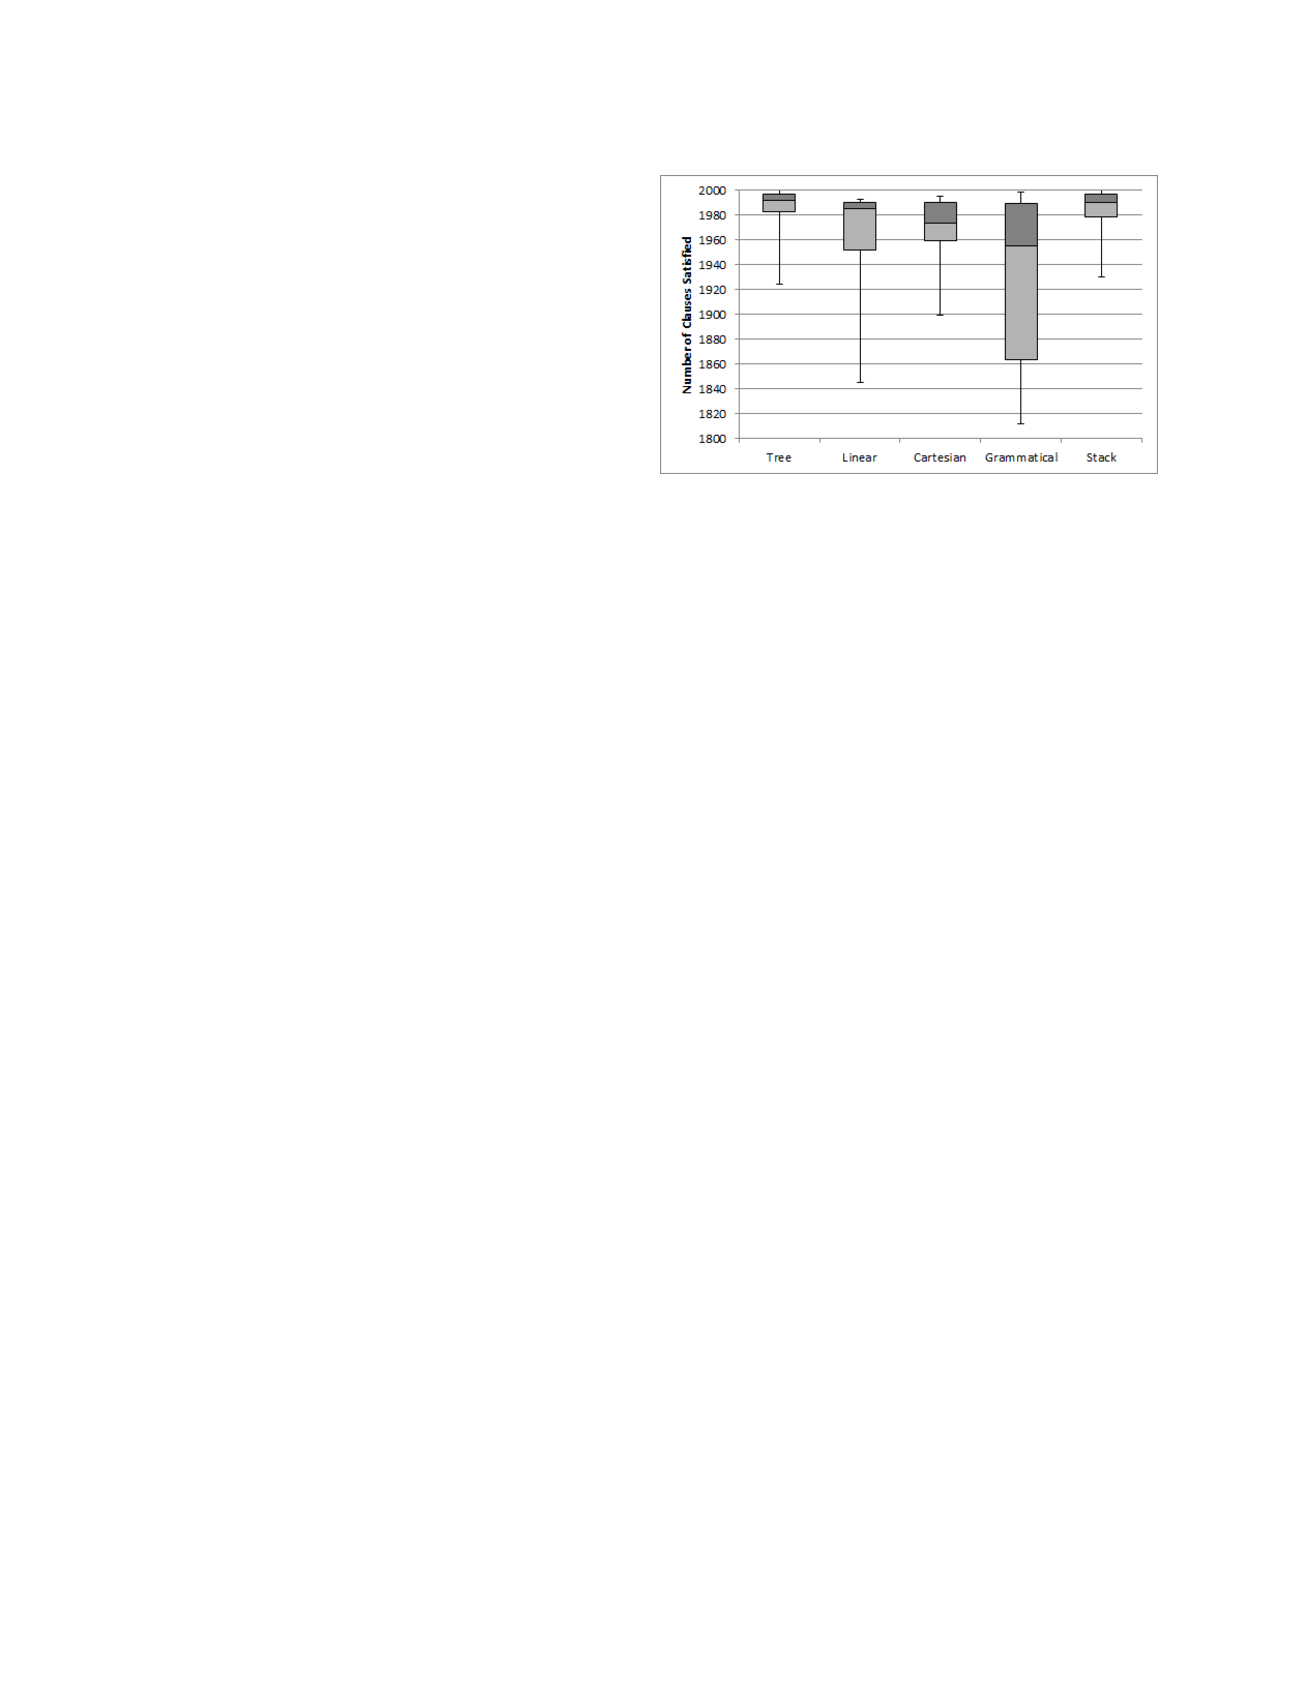
\psfig{file=gpvariant_graph.pdf,width =3.2in}
	\caption{Box plot showing the average number of SAT problem clauses that are satisfied by the best individuals from each run on the test set~\cite{harris:2015}.}
	\label{fig:gpvariants}
\end{figure}
Each hyper-heuristic (which is the same except for the GP variant used) was first run 30 times on a separate set of 3-SAT problems to `train' the hyper-heuristic. Then, after each run, the best program generated by each hyper-heuristic was run on the test set of 3-SAT problems 3 separate times. There were 3 problems in the training set and 8 in the test set, each containing 2000 \textit{clauses}, or subproblems, and 500 variables (to be filled in with boolean values produced by the programs produced by each hyper-heuristic). The hyper-heuristic runs were terminated after 40 generations. These results are summarized in Figure~\ref{fig:gpvariants}.

The results from Harris et al.~\cite{harris:2015} show that the GP variant chosen has a significant impact on the success of the hyper-heuristic. Tree-based GP and stack-based GP performed the best and performed similarly to one another, solving more clauses of the SAT problem on average than the other GP variants. Linear and Cartesian GP performed similarly to each other, but were not quite as good. Grammatical Evolution performed the worst. This does not mean that tree and stack are inherently better than other GP variants~--~it means that GP variants have different strengths and some are more suited to certain problem spaces than others. More testing is needed to determine how the GP variant used can cause a hyper-heuristics system to excel.

\section{Autoconstruction}
\label{sec:ac}
Autoconstruction is a genetic programming hyper-heur\-istic that uses genetic programming to evolve programs which have heuristic functions available to them to design the best program possible for a problem. 

In most genetic programming hyper-heuristics, the individual programs are evolving, but everything else is specified by the engineer. This means engineers might set half the population to produce children through a mutation that inserts an element every ten elements in a program. Then they might set the other half to be generated by crossover where the first half of the code for a child comes from one individual and the second half comes from another individual. In autoconstruction, engineers don't specify how programs construct their offspring. Instead, the methods of variation are encoded into the programs that are evolving so that, as a program evolves, its variation methods also evolve. An example of this is provided in Section~\ref{sec:autodog}.

Prior work on autoconstruction has explored a variety of system designs, but, until recently, they have only been able to solve simple problems. A new system called Autoconstructive Diversification of Genomes~(AutoDoG) has broken this trend by solving a problem that many genetic programming systems have struggled with: Replace Space with Newline~(RSWN)~\cite{spector:2016}. This problem (defined in Section~\ref{sec:results}) is complex for GP systems because it involves multiple data types and multiple outputs.

In Section~\ref{sec:push}, we introduce Push, the programming language used by AutoDoG. In Section~\ref{sec:autodog} we highlight some key features of AutoDoG and in Section~\ref{sec:results} we go over AutoDoG's recent success.

\subsection{Push}
\label{sec:push}

\begin{table}
	\centering
	\begin{tabular}{|r|c|c|c|c|c|c|c|}
		\hline
		exec & 1 & 2 & `hi' & string\_length & integer\_add \\
		\hline
		\hline
		\multirow{2}{*}{string} & & & & & \\
		& & & `hi' &  &  \\
		\hline
		\multirow{3}{*}{integer} & & & & 2 & \\
		& & 2 & 2 & 2 & 4 \\
		& 1 & 1 & 1 & 1 & 1\\
		\hline
	\end{tabular}
	\caption{Each column shows an element on the :exec stack and the contents of the other two stacks after processing that element.}
	\label{tab:push}
\end{table}

Push is a stack-based programming language with a separate stack for each data type. This means, for example, that there is a stack for integers, a stack for strings, and a stack for booleans. There are as many stacks as there are data types and designers can actually create their own data stacks as well.

Autoconstruction was one of the driving forces behind the original design of Push; Push was developed specifically for program evolution~\cite{spector:2016}. Push programs are sequences of instructions, constants, and parentheses with only one syntax requirement: the parentheses must be balanced~\cite{lee:2001}. For example, \texttt{((1 `hello') 2 integer\_add string\_length integer\_gt)} is a simple Push program.

Instructions are executed by putting them on the \texttt{exec} stack. For example, assume all stacks are empty and assume a program says \texttt{(1 2 `hi' string\_\-length integer\_add)}. In Table~\ref{tab:push}, we illustrate the execution of this program (there are more types of data stacks, but we only use two for this example). We push the entire program onto the \texttt{exec} stack to start. We then push 1, 2, and `hi' onto their appropriate data stacks. The \texttt{string\_length} instruction takes a string off the \texttt{string} stack and returns the string-length, in this case 2. The \texttt{integer\_add} works like \texttt{add} in Table~\ref{tab:stacks}. If instructions do not have enough arguments, they are skipped (as described in Section~\ref{sec:sgp}).~\cite{lee:tutorial}

%Plush is a linear genome format for Push~\cite{spector:2016}. This means that Plush is a format of the Push language that allows the programs to be stored in linear genomes. \textit{Linear genomes} are an example of an artificial chromosome (see Section~\ref{sec:GP}). In Section~\ref{sec:autodog}, AutoDoG is actually evolving linear genomes and then translating those genomes back into Push programs~\cite{spector:2016}. This allows for methods of variation in a population to be encoded and evolved more easily. We can just think of genomes as the structure which holds programs for the reproduction process.

\subsection{AutoDoG}
\label{sec:autodog}

\begin{figure*}
	\centering
	\begin{minipage}[b]{0.4\textwidth}
		%\psfig{file=dlstandard.pdf,width =3in}
		\includegraphics[width=\textwidth]{dlstandard.pdf}
		\caption{DL-distances between parent and child during a single PushGP run on RSWN~\cite{spector:2016}.}
		\label{fig:standard}
	\end{minipage}
	\hfill
	\begin{minipage}[b]{0.4\textwidth}
		%\psfig{file=dlac.pdf,width =3in}
		\includegraphics[width=\textwidth]{dlac.pdf}
		\caption{DL-distances between parent and child for a single autoconstructive run on RSWN~\cite{spector:2016}.}
		\label{fig:ac}
	\end{minipage}
\end{figure*}

In this Section, we briefly describe some of the key features of AutoDoG, designed by Spector et al~\cite{spector:2016}.

%When designing AutoDoG, Spector et al.~\cite{spector:2016} wanted to maintain diversity in parent selection. To do this, AutoDoG uses Lexicase Selection. Its name comes from the way it filters the population using a kind of ``lexicographic ordering" of cases. When tested on a benchmark suite of problems taken from introductory programming textbooks and compared to the results of other current GP parent selection techniques, Lexicase Selection allows for the solution of more problems in fewer generations.

AutoDoG works similarly to PushGP, a reasonably standard genetic programming system, but is run with autoconstruction as the sole genetic operator rather than using human designed operators like muatation and crossover. In PushGP, the methods for generating children (in the reproduction phase) are set by the designers, but in AutoDoG this is not entirely the case. Spector et al. created building blocks for generating children within AutoDoG's instruction set, but the rates at which these building blocks are used and how they are combined into higher level operations changes throughout the evolution of programs. One example of a building block would be \texttt{genome\_uniform\_addition}; this is an instruction which inserts random elements into a program with a likelihood taken from the top of the \texttt{float} stack~\cite{clojush}. The number at the top of the \texttt{float} stack changes as a program executes; so depending on where the \texttt{genome\_unif\-orm\_addition} occurs in the program, the rate of element insertion may be very different between programs.~\cite{spector:2016}

There is an ongoing discussion about how much guidance to give the AutoDoG system. Some of the designers think building blocks like \texttt{genome\_uniform\_addition} are giving the system too much instruction~--~some think we should not give any building blocks and should let AutoDoG evolve all instructions from scratch. The problem with evolving everything from scratch is that the system would take much longer to develop solutions and may not develop solutions at all.~\cite{lee:2001,clojush,spector:2016}

In AutoDoG, the reproduction process works as follows:
A program that has performed well on the fitness tests has been selected\footnote{There is a complex method called Lexicase Selection used for this process (see Spector et al.~\cite{spector:2016}).} for reproduction. We will call this program Mom. Another program has also performed well and is selected~--~we will call this program Dad. The code from both Mom and Dad's programs is pushed onto the \texttt{genome} stack. The \texttt{genome} stack was created so that program code could be classified as a type of data; this allows programs to manipulate a copy of their code without breaking during the reproduction process.\footnote{There are actually these things called genomes which hold the program code. These genomes are what gets pushed onto the \texttt{genome} stack (see Spector et al.~\cite{spector:2016}).} Since Mom was selected first, Mom is run with the purpose of making a child. Part of Mom's code is dedicated to reproduction~--~for example, she may have \texttt{genome\_uniform\_addition} in her code which would take her program code off the \texttt{genome} stack and insert new code into it. Mom uses her reproduction code, which may or may not take pieces of Dad's code, and Mom makes code for a new program. This new code, which sits on top of the \texttt{genome} stack, is the child of Mom and Dad.

Once this child is constructed, there is the question of whether or not it will be passed on to the next generation. Spector et al.~\cite{spector:2016} was especially concerned about cloning when designing AutoDoG. \textit{Cloning} is when a parent makes a child that is an exact copy of the parent and this child moves on to the next generation. This is a major concern with evolutionary systems because, if a program performs well enough on the fitness tests to move to the reproduction phase, making a child that is an exact copy allows this child to perform equally well on the fitness tests (and is therefore a good strategy). Most programs do this if allowed because changing the code is risky; if the change is for the worse, then the program's child will not pass the fitness tests given to the next generation. This means the child would not get to move to the reproduction phase and would therefore not pass its code on to the following generation. Cloning is a good strategy to pass fitness tests, but, from an engineer's perspective, cloning is bad; this because it prevents the system from exploring a wide range of possible solutions, which makes it difficult to find the global optima. It also significantly slows down the rate of evolution.

Most autoconstruction systems have some form of the ``no cloning rule," and AutoDoG has a form of this as well. AutoDoG's version of this requires offspring to pass a more stringent diversification test in order to enter into the next generation. To describe this test, we will use the child created by Mom and Dad earlier~--~we will call this child ``Pat." This test begins by having Pat take itself as a mate (the way Mom took Dad as a mate). Pat is run a few times with the purpose of making children~--~Pat may manipulate its own code or take code from its mates to do this. Pat finishes running and the results are several children. If these children differ enough from Pat and from each other, Pat will be inserted into the next generation and the children will be discarded. If Pat fails this test, the test is repeated on a new, randomly generated program. If this random program passes, then this random program will move into the next generation. If this random program fails, then a completely empty program, with no code in it, is generated and inserted into the next population.\footnote{There is the danger of a population with mostly empty programs, but there are restrictions and constraints within AutoDoG to prevent this from becoming a problem~\cite{spector:2016}.} This empty program does not undergo the diversification test.
This test allows for a more diverse set of potential solutions and allows for greater exploration of the problem space.~\cite{spector:2016}

\todo[inline, color=green]{Left of here DO NOT GO REREAD BEFORE THIS, YOU HAVE REREAD 20 TIMES, IT'S OKAY.}
\subsection{Results of AutoDoG}
\label{sec:results}
One challenging problem AutoDoG has solved is Replace Space with Newline~(RSWN). This problem is taken from introductory level textbooks and is part the general program synthesis benchmark suite of problems used to evaluate how successful a GP system is~\cite{helmuth:2015}. A solution of RSWN is a program that takes in a string and prints that string with all spaces replaced by newlines; it also must return the integer count of the non-whitespace characters~\cite{helmuth:2015}. This is complex for GP systems because it involves multiple data types, such as strings and integers, and multiple outputs.

AutoDoG solves the RSWN problem 5--10\% of the time, whereas PushGP solves it about 50\% of the time~\cite{helmuth:2015}. Why do we consider this a success when a relatively standard GP system performs much more reliably? We consider it a success because autoconstruction automates more of the algorithm design process than other GP systems. So while it may not perform as well on RSWN, AutoDoG performs extremely well on the problem of automating algorithm design. AutoDog's success may not seem like much, but the fact that AutoDoG solves the problem at all is actually quite impressive; it is not surprising that AutoDoG performs less reliably because AutoDoG has to learn how to construct offspring as well as learn how to solve problems.

AutoDoG is unique among autoconstructive systems in that it can solve problems that are challenging for other autoconstructive systems.\footnote{Note that these problems are not difficult for people to solve~--~they are problems taken from introductory level textbooks~--~but they are difficult for GP systems to solve.} However, as stated by Spector et al.~\cite{spector:2016},
\begin{quotation}
	We do not know which of these [AutoDoG's features], or which combinations of these, may be responsible for the fact that AutoDoG appears to be capable of solving more difficult problems than previous autoconstructive evolution systems.
\end{quotation}
This is because it's hard to separate the pieces; there are a lot of intertwined elements of AutoDoG and Push. Separating them to find exactly which elements contribute to the success without unraveling the entire system is difficult and has not yet been accomplished.

One interesting thing to note about AutoDoG is how it evolves. In standard PushGP, there is not a lot of change in Damerau-Levenshtein distance~(DL-distance) in Figure~\ref{fig:standard}. A \textit{Damerau-Levenshtein distance} can be thought of as a measure of change between the code of a parent and code of a child over the course of a single generation. In Figure~\ref{fig:standard}, over the 150 or so generations, change occurs at a steady rate and is not very dramatic from one generation to the next~--~the most change that occurs is about 200 differences between a parent and child, and the distances is often much smaller than that (the scattered dots near the first generation occurs because the first set of individuals is randomly generated). This is because engineers create a fixed set of reproduction mechanisms before they run the program. On the other hand, there are big differences between the code of some parents and their children as shown in the AutoDoG run shown in Figure~\ref{fig:ac}. Notice how the y-axis goes up to 2500 DL-distance in the AutoDoG graph compared to only about 800 in the PushGP graph. This is due to the fact that, in AutoDoG, the programs are evolving their reproduction mechanisms. In the AutoDoG graph, we are essentially seeing evolution evolve.

\section{Conclusions and Future Work}
\label{sec:conclusion}
Automating algorithm design is a complex problem that has been investigated for over 60 years. We have recently automated more of the algorithm design process through the use of genetic programming hyper-heuristics, specifically using a technique called autoconstruction. Systems like AutoDoG are important because they bring us closer generating algorithms from scratch. This could mean we would not need programmers to write simple algorithms anymore because the computer would do this job for us; this could drastically change the programming industry.

However, according to Pappa et al.~\cite{pappa:2014} in 2014, machine learning was ahead of hyper-heuristics development on the subject of automating algorithm design and ``can operate over different datasets, from different problem domains, and even with different features." This is not to say that machine learning is better than hyper-heuristics; the two have different methodologies and ways of approaching the problem of automating algorithm design. Pappa et al. states that the next step is working on getting hyper-heuristic development to the same level. They state that both heuristic and algorithm selection/generation are useful for all types of domains in which many parameters and methods are available, but no clear criteria or methodology exists for selecting them.

It would be interesting to see machine learning techniques combined with hyper-heuristics. Cartesian genetic programming (one of the GP variants in Harris et al.~\cite{harris:2015}) has a similar structure to neural networks, a type of machine learning technique. It might be interesting to try and combine the two structures to automate more of the algorithm design process.

\section*{Acknowledgments}
\label{sec:acknowledgments}
Special thanks to Nic McPhee and Elena Machkasova for their time, feedback, and constructive comments. And thanks to Alex Jarvis and Michael Bukatin, my external reviewers.


% The following two commands are all you need in the
% initial runs of your .tex file to
% produce the bibliography for the citations in your paper.
\bibliographystyle{abbrv}
% browning_paper.bib is the name of the BibTex file containing the
% bibliography entries. Note that you *don't* include the .bib ending here.
\bibliography{browning_paper}  
% You must have a proper ".bib" file
%  and remember to run:
% latex bibtex latex latex
% to resolve all references

\end{document}